\subsection{BGD, SGD, MBGD}
神经网络的训练过程, 可以看作目标函数的优化过程, 在优化过程中对模型的参数进行更新, 使目标函数逐步收敛到一个最优的状态. 参数优化有多种方法, 目前主要是基于迭代的过程, 如梯度下降、牛顿法等. 其中梯度下降已经霸榜多年. 目前主要有以下三种梯度下降方法: 
\begin{myitemize}
	\item BGD, Batch  Gradient Descent, 批量梯度下降. 每次计算梯度时使用全量样本. 优点: 
	\begin{myitemize}
		\item 所有样本都参与了梯度的计算, 异常样本带来的影响更小, 训练过程更稳定
		\item 收敛速度快
	\end{myitemize}
	缺点也很明显, 因为使用到了所有样本, 故计算耗时更长, 且要将数据全部加载, 对资源要求更高, 且有可能收敛到局部最优. 
	
	\item SGD, Stochastic Gradient Descent, 随机梯度下降. 每次计算梯度时只使用一个样本, 通常会对全量数据进行打乱. 优点: 
	\begin{myitemize}
		\item 参数更新频次高, 速度快. (但从另一个角度来看, 单独计算每个样本的梯度或许更耗时)
		\item 可以在线优化
		\item 每次使用一个样本的随机性可能会帮助跳出局部最优
	\end{myitemize}
	缺点: 每次只是用一个样本, 会放大一场样本的影响, 导致训练过程不稳定. 
	
	\item MBGD, Mini-Batch Gradient Descent, 小批量梯度下降. 每次使用一部分数据计算梯度, 一次通常将全量数据划分成多个batch, 与SGD类似, 也会对全量数据进行打乱. 优点: 
	\begin{myitemize}
		\item 对比BGD, 速度更快, 对资源要求更低;对比SGD, 振荡现象没有那么明显, 比SGD会更稳定
		\item 能够一定程度避免异常样本的干扰
	\end{myitemize}
	缺点: 需要考虑学习率的衰减, 以及选择合适的batch size, 且与BGD相比存在一定程度的振荡. 
\end{myitemize}
参考资料: \href{https://lumingdong.cn/summary-of-gradient-descent-algorithm.html#%E6%A2%AF%E5%BA%A6%E4%B8%8B%E9%99%8D%E7%AE%97%E6%B3%95%E7%9A%84%E4%B8%89%E4%B8%AA%E5%8F%98%E7%A7%8D}{梯度下降算法的三个变种}. 

\subsection{Normalization}
\subsubsection{Batch Normalization}
在神经网络中, 前一层的输出会成为后一层的输入. 当前面层的参数更新后, 其输出的分布也会随之改变, 经过层层的叠加, 越往后的变化越大. 为了拟合这些数据, 深层的参数需要不断适应变化的数据, 导致模型的\textbf{收敛速度很慢}. 这里的分布指的是一层里每个神经元的分布. 这种分布不一致做 \textbf{Internal Convariate Shift}(内部协变量偏移). 对于一个神经元, 其取值分布会逐渐偏移, 例如偏移至激活函数的饱和区, 即梯度很小. 

一个比较直观的方式就是对每一层的输出进行标准化. Batch Normalization 在 mini-batch 的基础上对每个神经元进行标准化, 即对每个特征进行标准化. 具体操作为: 每一层的输入为一个 mini-batch, 通过这个批次来估算每一维的均值和方差, 然后对每一维进行标准化, 除此之外, BN 中还对标准化后的特征进行了线性变化. 
$$
\begin{array}{rlr|}
	\hline \text { Input: } & \text { Values of } x \text { over a mini-batch: } \mathcal{B}=\left\{x_{1 \ldots m}\right\} \\
	& \text { Parameters to be learned: } \gamma, \beta & \\
	\text { Output: } & \left\{y_{i}=\operatorname{BN}_{\gamma, \beta}\left(x_{i}\right)\right\} & \\
	\mu_{\mathcal{B}} & \leftarrow \frac{1}{m} \sum_{i=1}^{m} x_{i} & \multicolumn{1}{l|}{\text { // mini-batch mean }} \\
	\sigma_{\mathcal{B}}^{2} & \leftarrow \frac{1}{m} \sum_{i=1}^{m}\left(x_{i}-\mu_{\mathcal{B}}\right)^{2} & \text { // mini-batch variance } \\
	\widehat{x}_{i} & \leftarrow \frac{x_{i}-\mu_{\mathcal{B}}}{\sqrt{\sigma_{\mathcal{B}}^{2}+\epsilon}} & \text { // normalize } \\
	y_{i} & \leftarrow \gamma \widehat{x}_{i}+\beta \equiv \mathrm{BN}_{\gamma, \beta}\left(x_{i}\right) & \text { // scale and shift }
\end{array}
$$
注意上面公式中是以一个特征维度为例子, 对于其他维也是一样的, 其中的 $\gamma, \beta$ 都是需要学习的参数, 即每个神经元会多出来两个参数来学习. 上述过程是在针对训练而言的, 但是在推断时该怎么办呢?对于测试数据, 依然会进行标准化($\gamma, \beta$ 是在训练时学习好的, 所以推断时是会被固定的), 但是其均值和标准差就不是通过批次数据来计算的, 而是这样: 
$$
\begin{aligned}
	\mathrm{E}[x] & \leftarrow \mathrm{E}_{\mathcal{B}}\left[\mu_{\mathcal{B}}\right] \\
	\operatorname{Var}[x] & \leftarrow \frac{m}{m-1} \mathrm{E}_{\mathcal{B}}\left[\sigma_{\mathcal{B}}^{2}\right]
\end{aligned}
$$
那么测试数据的标准化就是这样的: 
$$
\widehat{x}=\frac{x-\mathrm{E}[x]}{\sqrt{\operatorname{Var}[x]+\epsilon}}
$$
\textbf{为什么标准化后还要进行线性变换呢?}如果只是进行标准化后, 其很有可能落在激活函数的线性区域, 例如 sigmoid 激活函数, 经过标准化后基本会落在 0 左右, 而这一块区域基本是线性的, 而达不到激活函数的非线性的功能, 因此对齐进行了缩放和偏置, 使其能够落在激活函数的非线性区域, 由于 $\gamma, \beta$ 是学习得到的, 因此也能满足其落在线性区的需求. 这样做的一个目的就是: 保障每一层的表征能力. 

有一些观点认为 BN 有防止过拟合的作用, 给出的解释是: BN 将输入拉到了同一个分布, 且保证了输入不会都落到激活函数的饱和区, 可以使得参数的更新更加平滑, 也就达到了防止过拟合的作用. 


实际情况在进行BN时, 可能是在通过激活函数之前进行 BN 或者在通过激活函数后再进行BN. \textbf{通常是在激活函数之前进行 BN}, 因为当输入较大时, 通常激活函数的变化都较小, 梯度变化不明显, 故在激活函数之间就对数据进行BN, 使其分布尽量稳定. 

BN 的一些缺点: 
\begin{itemize}
	\item 需要较大的batch以体现整体数据分布, 要求 bath 的分布尽量与总体分布相近;
	\item 训练阶段需要保存每个batch的均值和方差, 以求出整体均值和方差在infrence阶段使用;
	\item 不适用于可变长序列的训练, 如RNN. 
\end{itemize}

\subsubsection{Layer Normalization}
既然已经有了 BN, 怎么还来了 LN 呢?参看 BN 的缺点, 其中很重要的一点就是不适用于处理序列数据的网络, 序列数据的格式通常为 $(batch\_size, seq\_len, emb\_dim)$, 但是$seq\_len$ 并不都是相同的. 如果对序列数据进行 BN, 则需要计算每个 $time\ step$ 上每个特征的均值和方差, 但是由于序列的长度是不一致的, 若遇到了没有在训练集中出现过的序列长度则无法对超出的 $time\ step$ 做 BN 了. 

与 BN 类似, LN 也是进行标准化后再进行线性变化. 不同点在于 LN 的标准化是针对层而言的, 而 BN 的标准化是针对神经元而言的. 具体做法: LN 计算层中所有神经元的均值与方差, 对于一个 batch 而言, 则会计算出 $(batch\_size, seq\_len)$ 个均值和方差, 即序列中每个元素(维度为 $emb\_dim$ 的向量)一对均值和方差, 然后对同一层使用相同的均值和方差做标准化后进行线性变化即可. 
$$
\mu^{l}=\frac{1}{H} \sum_{i=1}^{H} a_{i}^{l} \quad \sigma^{l}=\sqrt{\frac{1}{H} \sum_{i=1}^{H}\left(a_{i}^{l}-\mu^{l}\right)^{2}}
$$
其中 $a_i^l$ 就是第 $l$ 层的第 $i$ 个神经元, $H$ 是隐层的单元数. 可以看到, 计算的过程中不用考虑 batch 的大小, 因此 batch 的大小和选择对 LN 是没有影响的. 进行缩放时则与 BN 是一致的, 每个神经元都有单独的缩放系数和偏置. 因为不受 batch 中其他样本的影响, 因此使用 LN 时不需要保存训练过程中各个 batch 的均值和方差, 且训练过程和推断过程 LN 的操作是一致的. 

\subsection{Dropout}
Dropout 即丢弃, 是神经网络中一种正则化的手段: 在神经网络模型做训练时, 让网络中某些神经元随机失活——也就是不参与训练. 换个角度理解一下这个操作背后的含义: Dropout使得每批训练数据进入神经网络时, 神经网络的构型都不同, 即每批训练数据训练的网络结构都不同. 而做预测Dropout是关闭的状态, 代表着\textbf{做预测时是所有训练时结构不同的神经网络一起做的最后的预测, 整个过程就是多个不同神经网络最后投票做决定给出预测值}. 其实可以看到这和随机森林的 \textbf{bagging} 很像了. 

参考 PyTorch 中关于 Dropout 的实现: \ref{nn_dropout}. 

\subsection{Model Collapse}
模型坍塌, 很形象啊, 就是模型出现了一个漏洞, 不管你输入什么东西都会漏进这个洞里. 

这个主要出现在GAN的模型中. GAN通过生成器G和判别器D来使G捕捉到真实数据的分布. 在训练GAN模型时会出现model collapse的现象, 即G只捕捉到了真实数据的部分分布. 为什么会这样呢?简单的介绍一下: 当G捕捉到了真实数据的部分分布后, 被D识破了, 于是G就改变, 从某个分布跳到了另外的分布, 并且抛弃了原来的分布, 于是就成了“猫鼠游戏”, D一直追着G跑, G最终并没有完全捕捉到真实数据的分布. 参考: \href{https://blog.csdn.net/SPARKKKK/article/details/72598041}{GAN——ModeCollapse}. 


\subsection{关于CNN的一点理解}
于DNN相比, CNN有两个特点: 1)局部感知;2)权值共享. 

局部感知. 在CNN中每个Feature map中的一个值只于上一层的Feature map的一小部分有关. 如果将CNN展开成DNN的形式, 则一层中的一个神经元的输入只是上一层的某几个神经元. 与全连接不同, 全连接将上一层的所有信息作为输入, 捕捉整体的信息. 但局部感知以某个区域内的信息作为输入, 捕获上一层数据中存在的局部信息 --- 特定的模式. 

权值共享. CNN中的每一个filter都可以得到一个Feature map, 同一个Feature map中的元素之间通过同一个filter卷积得到. 或者说, 同一层的神经元由一个filter产生, 共享一套参数. 
见Fig.\ref{fig:share_weight}. 图来源于李宏毅老师的ppt. 有一点需要注意, CNN模型的输入图像可能是单通道的也可能是三通道的, 此时\textbf{每个filter不仅由长和宽还有深度}, filter的深度与图像的通道数是相等的, 所以一般来说有多少个filter就有多少个Feature map. 

\begin{figure}[h]
	\centering
	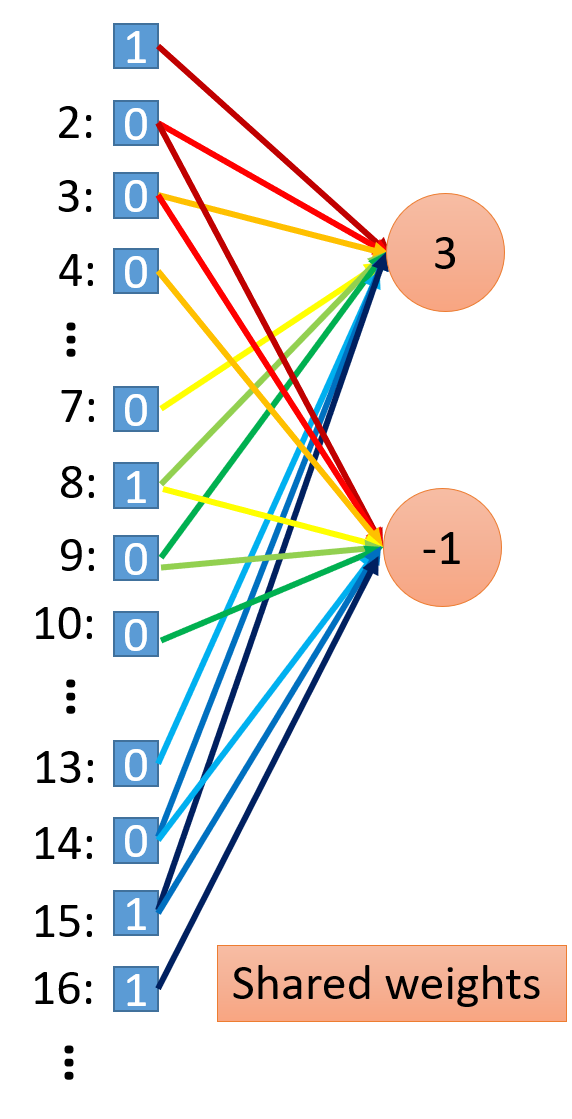
\includegraphics[width=.3\textwidth]{pics/share_weight.png}
	\caption{CNN的权值共享}
	\label{fig:share_weight}
\end{figure}

CNN的应用非常广泛, 不仅是图像, 在Speech、NLP等很多领域都有非常多的应用. 在决定是否要使用基于CNN的模型时, 需要考虑: 1)数据中存在一些较小的模式, 这些模式经常出现在数据中 --- 对用卷积核;2)模式与整个数据相比比较小, 更大的语义信息是由很多小的模式组成的;3)进行pooling时不会破坏数据本来的含义. 

在探索CNN到底学习到了什么的时候, 可以在训练好模型后, 通过不断优化输入的数据, 来检验是什么样的输入使得基于CNN的模型中的神经元能够得到最大的激活 --- 什么样的输入使神经元最兴奋. 这些主要涉及到对CNN的解释和可视化. 

\subsection{深度学习中常见的参数初始化方法}
深度学习依靠大量的数据进行学习能够达到很好的效果, 但是这其中依靠的是大量的参数, 学习就是为这些参数找到合适的值. 因此, 如果一开始我们就能给这些参数设置一个比较好的值, 那么学习也就省力了, 这也就是如何初始化的问题了. 

\subsubsection{从正态分布中采样}
或许直接将参数初始化为 0 也能进行学习, 但是容易存在一些问题: 学习过程缓慢, 难以收敛, 学习效果不好, 为什么呢?如果参数全为 0, 则计算的损失可能会很小, 能够提供的梯度值也会很小或者根本就等于 0, 这对于依靠梯度更新参数的方法来说是很致命的. 因此, 与全 0 相比, 随机初始化反而是一个不错的选择, 至少不会让梯度为 0. 

\subsubsection{Glorot initialization}
但是呢, 从正态分布中采样也不是一个很好的方法, 为什么呢?将设我们从 $\mathcal{N}(\mu, \sigma^2)$ 中采样权重, 参数的方差会影响隐层的线性变换后的方差, 进而影响隐层输出的方差, 这会直接影响梯度的计算, 如以 sigmoid 为激活函数时, 则可能落在平坦的区域 --- 也就是可能会出现梯度向后传着传着就没了或者就变得很大了. 

因此一个好的初始化应该满足: 各层的值(线性变换后的值、激活后的值)应该有相似的方差. 为了满足前向传播时各隐层的输出值有相似的方差, 以及在反向传播时, 梯度也具有相似的方差, 我们可以推导出参数应该又怎样的方差, 这其中涉及到一些数学推导, 暂时不展开. 结论就是, 为了前向的稳定, 参数的方差应该是 $\frac{1}{f_{in}}$, 为了反向传播的稳定, 参数的方差应该为 $\frac{1}{f_{out}}$, 其中 $\boldsymbol{W}^{fan_{in} \times fan_{out}}$. 那这里有两个方差怎么办: 取平均, 即 $Var(\boldsymbol{W}) = \frac{1}{ \frac{fan_{in} + fan_{out}}{2}}  = \frac{2}{fan_{in} + fan_{out}}$. 因此如果我们从正太分布中采样, 则这个正太分布的方差应该等于 $\frac{2}{fan_{in} + fan_{out}}$, 均值应该等于 0, 为啥呢?在推导过程中利用了方差的一些性质, 要求均值为 0. 如果从均匀分布 $U(a, b)$ 中采样呢?同样需要满足 0 均值, 即 $a + b = 0$, 那等于多少呢?因为均匀分布的方差为 $\frac{(b - a)^2}{12}$, 且 $a = -b$, 因此可以解得 $b = \sqrt{\frac{6}{fan_{in} + fan_{out}}}$. 

上述方法就是Xavier初始化方法(又称Glorot初始化). 当然, 初始化方法还要考虑激活函数的影响, Glorot 主要用于输出均值为 0 的激活函数, 如 tanh. 

\subsubsection{He 初始化}
如果使用 ReLu 作为激活函数, 上述的 Glorot 可能就不是那么好了, 为什么呢?考虑 $ReLu(x) = max(0, x)$, 将隐层的输出近一半置为 0, 且 ReLu 的输出均值不为 0, 不满足 Glorot 推导过程中的一些条件. 为了满足各层的值方差就近似, He 初始化对权重的方差变为了 Glorot 中的两倍, 为什么呢?因为 ReLu 将一般元素的值置零相当于减少了一半方差. He 初始化没有同时使用 $fan_{in}, fan_{out}$, 而只使用了其中一个, 实验表明这已经足够了. 因此, 使用 He 初始化时, 正态分布的方差为 $\frac{2}{fan_{in}}$, 均匀分布的的 b 为 $\sqrt{\frac{6}{fan_{in}}}$. 

关于推导的一些参考: \href{https://intoli.com/blog/neural-network-initialization/}{UNDERSTANDING NEURAL NETWORK WEIGHT INITIALIZATION}、\href{https://mnsgrg.com/2017/12/21/xavier-initialization/}{Xavier Initialization}(不同激活函数下的 Glorot 初始化推导). 


\subsection{DL中的不可微操作}

\subsection{Global Max Pooling}

\subsection{Attention机制与CNN}

\subsection{Batch Size与Learning Rate}
模型训练过程中, \textbf{Batch Size}和\textbf{Learning Rate}是两个不可不调的参数. 


\subsection{深度学习的梯度下降优化算法}
这里按照 PyTorch 里的优化器来进行介绍. 
\subsubsection{SGD}
\href{https://pytorch.org/docs/stable/generated/torch.optim.SGD.html#torch.optim.SGD}{SGD}(stochastic gradient descent), 就是常说的随机梯度下降, 当然在 PyTorch 的实现中, 可以加入一些额外的操作, 如: 权重衰减、动量(上一步的梯度呈指数加权来影响当前梯度). SGD 的计算过程如 Fig.\ref{fig:sgd} 所示. 

\begin{figure}[h]
	\centering
	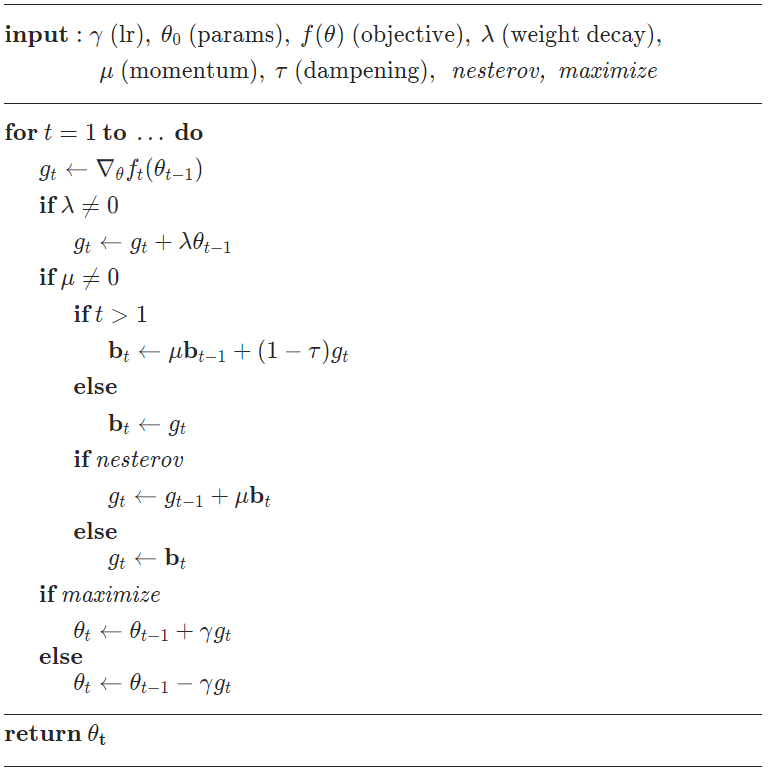
\includegraphics[width=0.6\textwidth]{pics/sgd.png}
	\caption{SGD 计算过程(\href{https://pytorch.org/docs/stable/generated/torch.optim.SGD.html#torch.optim.SGD}{来源})}
	\label{fig:sgd}
\end{figure}

SGD 的特点: 
\begin{itemize}
	\item 朴素的 SGD 最大的缺点是下降速度慢, 而且可能会在沟壑的两边持续震荡, 停留在一个局部最优点;
	
	\item 为了解决朴素 SGD 中的振荡现象, 可以加入动量;
	
	\item 对于稀疏数据集, 对所有参数使用相同的学习率是不太合适的, 每个参数更新的步长与特征的稀疏程度有关;
\end{itemize}

\subsubsection{AdaGrad}
即 Adaptive Gradient, 自适应梯度. 该算法通过记录迭代过程中梯度的信息来自动地调整学习率. 可以实现针对不同的参数自动调节学习率的大小. 其计算方式:

$$
w^{t+1} \leftarrow w^t - \frac{\eta}{\sqrt{\sum_{i=0}^t (g^i)^2}} \odot g^t
$$

可以看出, 随着迭代, 学习率是\textbf{单调递减}的, 且对于梯度较大的参数其更细你的步伐也更大. 其缺点为: 1) 从训练开始时累积平方梯度值会越来越大, 会导致学习率过早和过量的减少, 从而导致迭代后期收敛及其缓慢; 2) 需要手动设置全局学习率. 

\subsubsection{RMSProp}
即 Root Mean Square Prop, 该算法是 AdaGrad 的一种改进, 区别在于梯度累计的方式不同, 在 AdaGrad 中为累加梯度的平方, RMSProp 中则是引入了一个衰减系数来累加:

$$
r \leftarrow \rho r + (1 - \rho) g \odot g
$$
其中 $r$ 就是梯度累积量, 梯度更新方式与 AdaGrad 一样:

$$
w^{t+1} \leftarrow w^t - \frac{\eta}{\sqrt{r}} \odot g^t
$$

由于 $r$ 参考了历史的梯度信息, 因此在更新的过程中更稳定.

\subsubsection{AdaDelta}
AdaDelta 也是针对 AdaGrad 的一种改进. 与 RMWProp 不同, AdaDelta 不需要设置一个初始的学习率. 其计算过程如 Fig.\ref{fig:adadelta} 所示.

\begin{figure}[h]
	\centering
	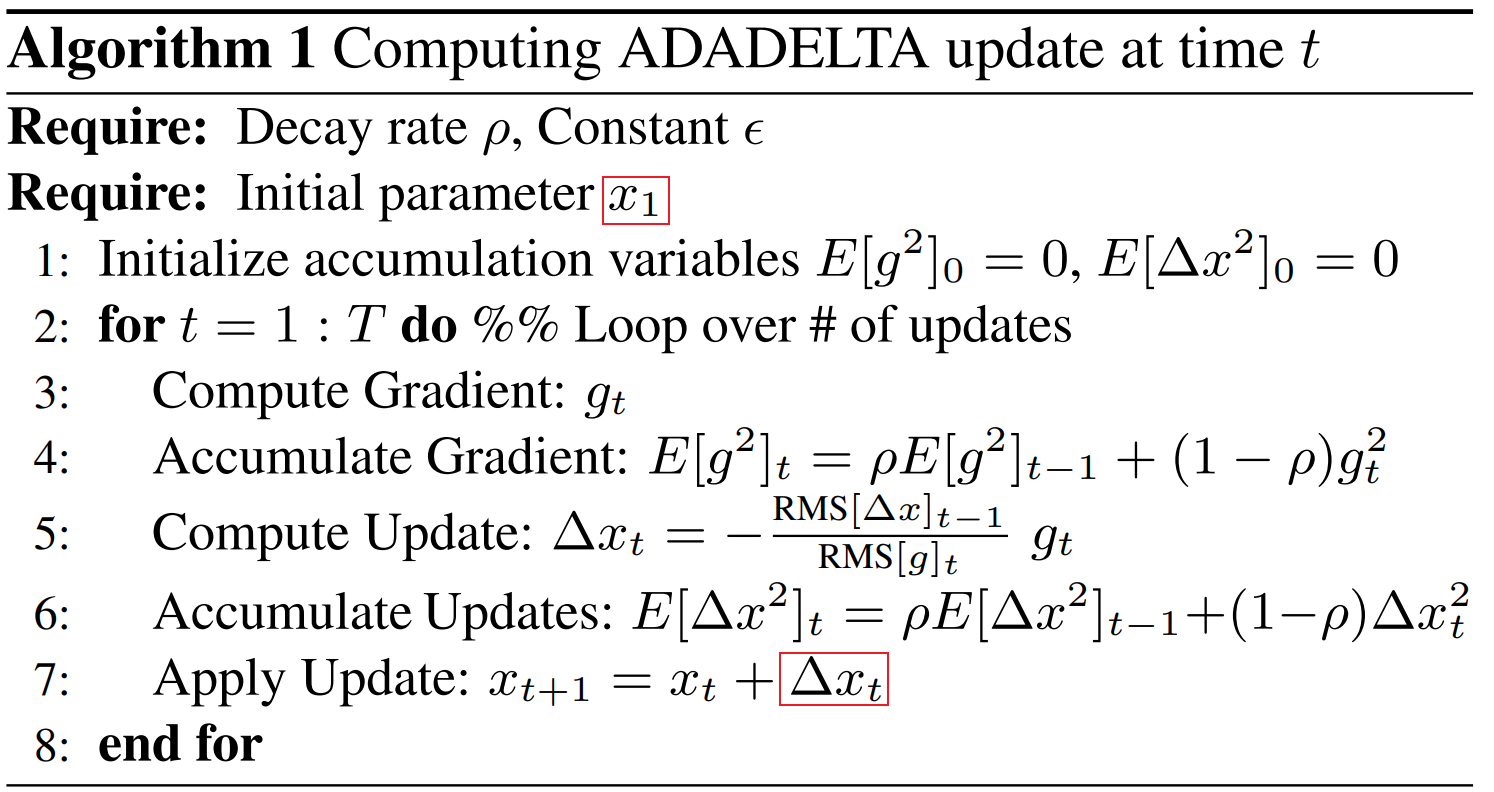
\includegraphics[width=0.8\textwidth]{pics/adadelta.png}
	\caption{AdaDelta 计算过程}
	\label{fig:adadelta}
\end{figure}

参数的更新量 $\Delta x_t$ (AdaDelta 中的 Delta 应该就是指 $\Delta x$)并不是通过学习率乘以梯度得到的, 而是一个指数加权平均的量. 与 RMSProp 相比, AdaDelta 相当于用上一步参数更新量的均方根近似学习率 ($\Delta x_t = -\frac{\text{RMS}[\Delta x]_{t-1}}{\text{RMS}[g]_t} g_t$). 

AdaDelta \textbf{特点}: 1) 不需要设置初始的学习率, 但是在一些深度学习框架中 (如 pytorch), 可以看到所实现的 AdaDelta 优化器还有学习率这个参数, 但是这个学习率是针对 $\Delta x$ 所做的缩放, 其取值也一般比较大; 2) 训练的早期和中期收敛速度快 (\textcolor{red}{从\href{https://arxiv.org/pdf/1212.5701.pdf}{论文}来看, $\Delta x$ 的更新类似于牛顿迭代, 使用了近似二阶信息, 所以收敛快}), 但是后期容易在局部最小值附近抖动.

\subsubsection{Adam}
Adam\cite{kingma2015adam} 结合 AdaGrad 和 RMSProp 两种优化算法的优点, 对梯度的一阶矩估计(First Moment  Estimation, 即梯度的均值)和二阶矩估计(Second Moment Estimation, 即梯度的未中心化的方差)进行综合考虑, 计算出更新步长. Adam 的计算过程如 Fig.\ref{fig:adam} 所示. 

\begin{figure}[h]
	\centering
	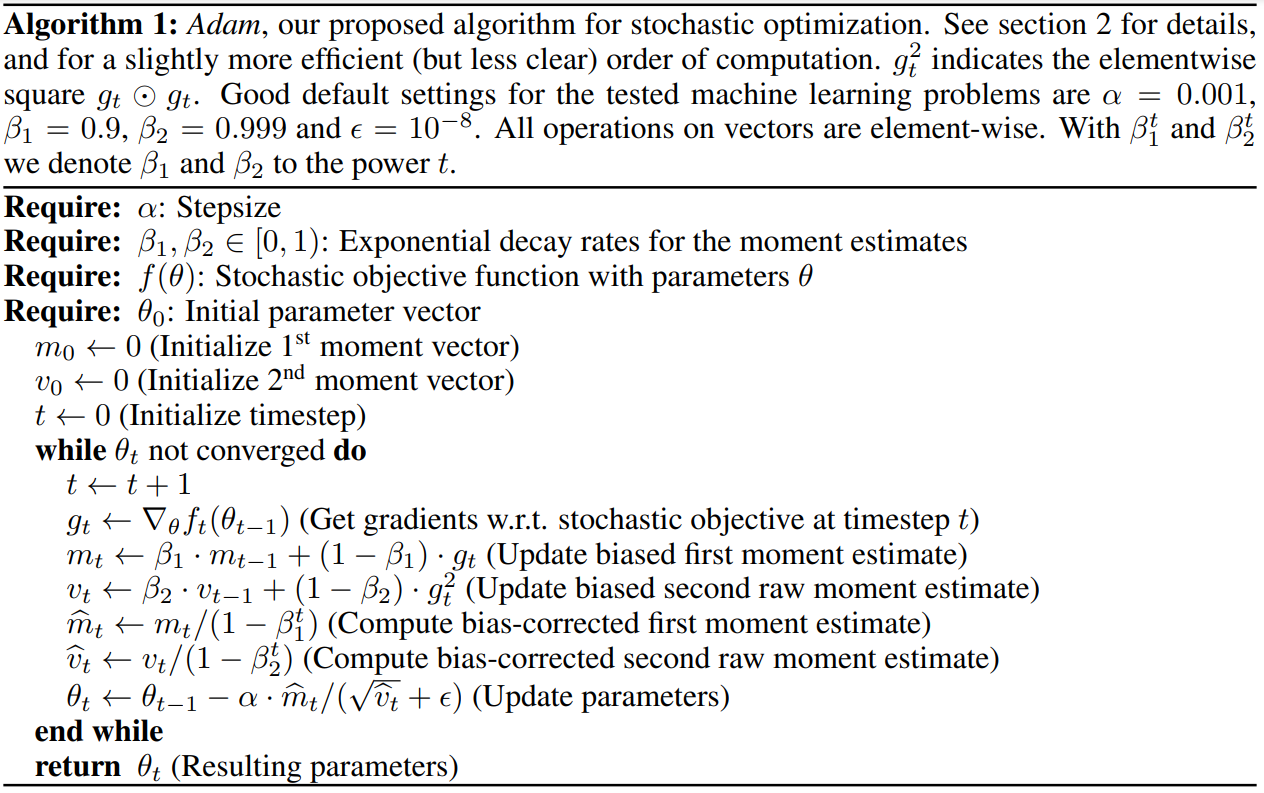
\includegraphics[width=0.8\textwidth]{pics/adam.png}
	\caption{Adam 计算过程}
	\label{fig:adam}
\end{figure}

可以看到计算完 $m_t, v_t$ 后又分别除以了 $1-\beta^t$, 随着 $t$ 的增大 $1 - \beta^t$ 逐渐接近 1. 为什么要这样呢? \textcolor{red}{由于 $m, v$ 的初始值都是 0, 在后续的估计中, $m, v$ 都会偏向于 0, 即 $m_t, v_t$ 不是 $E[g_t], E[g_t^2]$ 的无偏估计, 因此需要各自除以 $1 - \beta^t$, 具体的推到可以参考\href{https://arxiv.org/pdf/1412.6980.pdf}{论文}}.

网上找到一张梯度的一阶估计随时间步的变化(即 Fig.\ref{fig:adam} 中的 $m_t$), 如 Fig.\ref{fig:adam-gradient} 所示. 可以看到, 前面时间步的梯度在衰减. 
\begin{figure}[h]
	\centering
	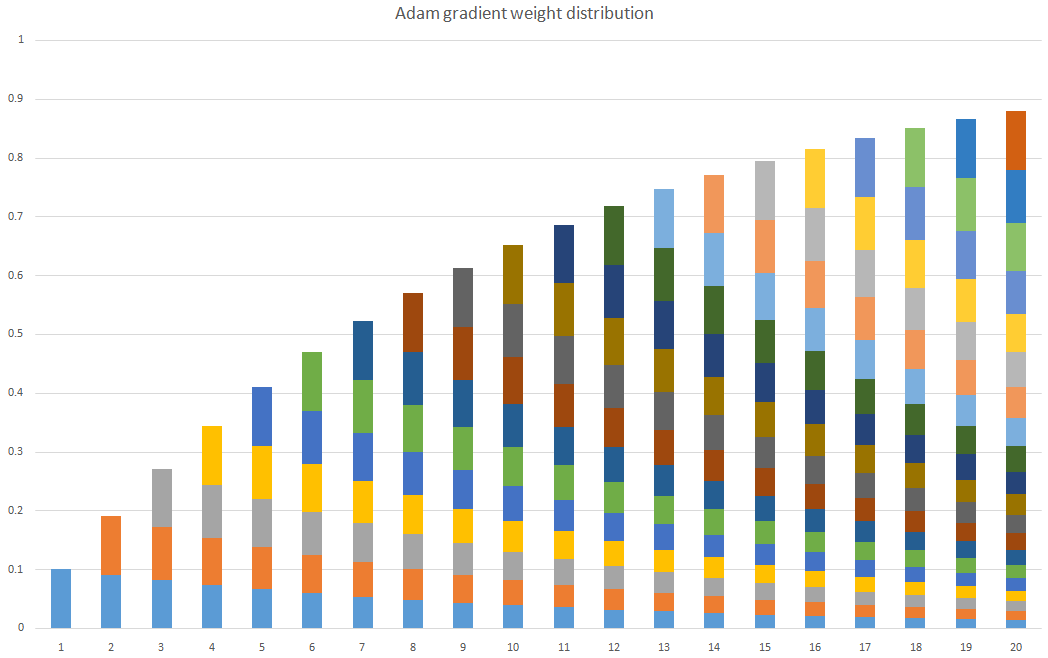
\includegraphics[width=0.85\textwidth]{pics/adam-gradient-weight-distribution.png}
	\caption{Adam 梯度一阶估计随时间步的变化(\href{https://www.jianshu.com/p/aebcaf8af76e}{来源})}
	\label{fig:adam-gradient}
\end{figure}

Adam 的特点: 1) 参数更新的步长与梯度的大小无关; 2) 对目标函数没有平稳要求; 3) 适用于大多非凸优化问题, 适用于大数据集和高维空间; 4) 由于 $m_t, v_t$ 可以看作是对固定时间窗口内梯度的估计, 因此可能出现梯度突变的情况, 导致后期学习率震荡, 导致模型无法收敛 (因为学习率不能收敛为 0). 

参考资料: 
\begin{itemize}
	\item \href{https://mp.weixin.qq.com/s/L9jCK5rtyq3fJZEBpLvagg}{从SGD到NadaMax, 十种优化算法原理及实现};
	
	\item 一篇讨论各种优化算法的论文:  \href{https://arxiv.org/pdf/1612.04010.pdf}{An empirical analysis of the optimization of deep network loss surfaces};
\end{itemize}

\subsection{常见损失函数及其特点}
\subsubsection{MSE}
MSE(mean squared error, 均方误差), 常用于回归任务中. 其形式较为简单: 
$$
l(y, \hat{y}) = (y - \hat{y})^2
$$
其中 $y, \hat{y}$ 分别为样本的真实值与预测值. MSE 的特点: 
\begin{itemize}
	\item 当 $|y - \hat{y}|$ 大于 1 时, MSE 会放大误差, 所以 MSE 容易受到异常点的影响;
	
	\item MSE 的梯度与误差的大小成正比;
\end{itemize}

\subsubsection{交叉熵损失函数}
常用于分类任务中. 最常见的莫过于而分类中的交叉熵损失函数了: 
$$
l(y, \hat{y}) = -(y \log \hat{y} + (1-y) \log (1-\hat{y}))
$$
其中 $y \in \{0, 1\}, \hat{y} \in (0, 1)$, $\hat y$ 表示样本为正样本的概率. 交叉熵更一般的形式为: 
$$
l(\boldsymbol{y}, \hat{\boldsymbol{y}}) = - \sum_{c=1}^K \boldsymbol{y}_c \log \hat{\boldsymbol{y}}_c
$$
其中 $\boldsymbol{y} \in \{0,1\}^K$ 表示样本所属的类别的 one-hot 编码, $\hat{\boldsymbol{y}}$ 是样本属于每个类别的概率(已归一化). 由于 $\boldsymbol{y}$ 是 one-hot 编码, 若样本的真实类别是 $c$, 则上式可简化为: 
$$
l(\boldsymbol{y}, \hat{\boldsymbol{y}}) = - \log \hat{\boldsymbol{y}}_c
$$
如果赋予了每个类别一个权重, 那么交叉熵损失可写为: 
$$
l(\boldsymbol{y}, \hat{\boldsymbol{y}}) = - \boldsymbol{w}_c\log \hat{\boldsymbol{y}}_c
$$
$\boldsymbol{w}_c$ 表示类别 $c$ 的权重. 

交叉熵损失的特点: 
\begin{itemize}
	\item 最后一层的权重更新时, 梯度与激活函数的导数无关, 不会因为输入落在饱和区而影响梯度的更新, MSE 则存在这个问题;
	
	\item 从交叉熵的式子中也可以看到, 计算损失时只利用到了在正确类别上的信息, 而其他类别的信息直接丢弃了. 这样可能会导致其他错误类别上的概率基本时一样的, 而忽略了其他类别之间的差异. 例如猫、虎、汽车的三个类别, 如果真实类别是猫, 那么直观上来看虎的概率还是应该大于汽车的概率的, 但交叉熵是将这些类别等同看待的, 忽略了类别见的差异和相关性;	
\end{itemize}

\subsubsection{Focal Loss}
Focal Loss(后续简称为 FL)为解决样本不平衡的问题, 更准确地讲, 是为解决难分类样本 (Hard Example) 和易分类样本 (Easy Example) 的不平衡问题. 对于样本不平衡, 其实通过上面的带权重的交叉熵损失便可以一定程度上解决这个问题, 但是在实际问题中, 以权重来解决样本不平衡问题的效果不够理想. 为什么呢?表面上是因为样本不平衡, 但实质上导致效果不好的原因也许并不是简单地因为样本不平衡, 而是因为样本中存在一些 Hard Example, 同时存在许多 Easy Example, Easy Example 虽然容易被分类器分辨, 损失较小, 但是由于其数量大, 它们累积起来依然于大于 Hard Example 的损失值, 因此我们需要给 Hard Example 较大的权重, 给 Easy Example 较小的权重. FL 是基于交叉熵损失的, 其定义为: 
$$
FL(\boldsymbol{y}, \hat{\boldsymbol{p}}) = -(1-\boldsymbol{p}) \log \boldsymbol{p}
$$

其中 $\boldsymbol{p}, \hat{\boldsymbol{p}}$ 均为向量, 后者表示预测的各个类别的概率:

$$
\boldsymbol{p}_i= \begin{cases}
		\hat{\boldsymbol{p}}_i & \text { if } \boldsymbol{y}_i=1 \\ 
		1-\hat{\boldsymbol{p}}_i & \text { otherwise }
	\end{cases}
$$

可以看到, 与交叉熵相比, FL 多了一个 $(1-\boldsymbol{p})$, 显然, 当模型对该样本分类的置信度越高 (体现为对正样本其预测概率很大, 对负样本预测概率很低), 则样本的损失越小(相比交叉熵更小), $(1-\boldsymbol{p})$ 可以起到样本权重的作用, 该值越小说明样本越容易被分类, 即为 Easy Example. 为了更好控制该权重, 改写 FL 为: 
$$
FL(\boldsymbol{y}, \hat{\boldsymbol{p}}) = -(1-\boldsymbol{p})^\gamma \log \boldsymbol{p}
$$
其中 $\gamma$ 为超参数, $\gamma=0$ 则为交叉熵损失, 一般取 2, $\gamma$ 越大 Easy Example 带来的损失就越小, 对 Easy Example 起到的抑制就越大. 如果再要处理样本不均衡的问题, 可以再加上类别权重, 则 FL 改写为: 
$$
FL(\boldsymbol{y}, \hat{\boldsymbol{p}}) = - \boldsymbol{\alpha} (1-\boldsymbol{p})^\gamma \log \boldsymbol{p}
$$
其中 $\boldsymbol{\alpha}$ 为类别权重向量. 

\subsubsection{Sampled Softmax}

\subsubsection{Contrastive loss, Triplet loss} 
都是一种损失函数. 

Triplet loss用于训练差异较小的数据, 常用于人脸识别中. 以这种函数为损失函数时, 输入的一个样本是一个三元组(anchor, positive, negative), anchor是随机选择的一个样本, 而positive和negative分别于anchor为同类/异类数据. 在学习时, Triplet loss的目的就是让anchor的表征与positive的表征尽量靠近, 与negative的表征尽量疏远. 那么对于一个样本来说, Triplet loss写成公式:  
$$
\mathcal{L} = max( ||f(a)-f(p)||_2^2 - ||f(a) - f(n)||_2^2 + \alpha )
$$
公式的含义也很明显, 尽量使类内数据相近, 类间数据相离. 

Contrastive loss是对比损失, 也叫zero-one损失, 主要用来处理孪生网络中的paired data的关系. 通常Contrastive loss的输入是两个样本, 且各自都有一个标签, Contrastive loss的目标就是: 如果两个样本同类, 则loss更小, 否则loss更大. 写成公式: 
$$
\mathcal{L} = d_{ij}^2 \cdot Y_{ij} + (1 - Y_{ij} )max(margin - d_{ij}, 0)^2
$$
其中, $d_{ij}$就表示样本i, j之间的距离, 这个可以有多种形式的定义, $Y_{ij}$表示样本i, j的标签是否相同, margin是一个阈值, 如果$d_{ij}$超过阈值则应该尽量把它们划分开. 

\subsection{常见激活函数及其特点}
\subsubsection{sigmoid}
\begin{center}
	\begin{tikzpicture}
		\begin{axis}[
			legend pos=outer north east,
			xlabel = $x$,
			ylabel = {$f(x)$},
			]
			\addplot[color=red] {1/(1+exp(-x))};
			\addlegendentry{$f(x) = \frac{1}{1+e^{-x}}$}
		\end{axis}
	\end{tikzpicture}
\end{center}
这个恐怕是无人不知无人不晓了吧, 通常用于将神经元得输出转化成一个概率值. 

优点: 梯度平滑、易求导. 缺点: 
\begin{itemize}
	\item 计算复杂, 在正向和反向传播过程中都涉及到幂运算和处罚;
	
	\item 当输入值处在平缓区域时(即较大或较小), 导数接近于零, 可能会导致梯度很小/为零, 不利于更新参数;
	
	\item sigmoid 的输出不是零中心的;
\end{itemize}

\textbf{怎么解决 sigmoid 的梯度饱和的问题呢?} 1) 在 sigmod 之前引入 BN 层. 通过 BN 层对输入数据的分布进行规范化, 使其能够落在 sigmoid 的梯度较大的区域. 2) 替换激活函数. 建议非输出层的激活函数选用 ReLU; 3) 在模型重加入残差模块; 4) 采用 pre-training+fine-tuning 的方式训练模型, 即一层一层地训练隐层, 最后再进行微调; 5) 增加门控机制, 类似于 LSTM 和 GRU 中的门控单元.

\subsubsection{ReLU}
Rectified Linear Unit, 整流线性单元, 这个算是与 sigmoid 齐名的激活函数了: 
$$
relu(x) = max(0, x)
$$
优点: 计算速度很快, 而且导数很稳定(在大于 0 的部分为 1), 不会因为导数很小使得连乘后梯度很小. 缺点: 因为当输入小于 0 时输出为 0 且梯度为 0, 这其实相当于抛弃了一部分信息, 而且由于导数为零, 可能某些参数不能得到很好地学习. 

显然, Focal Loss 能够针对 Hard/Easy 样本给出不同的权重. 

\subsubsection{Leaky ReLU}
可以看到在 ReLU 里, 当输入为 0 时输出直接为 0, 导数也为 0. Leaky ReLU 对输入小于 0 时进行了修改: 
$$
Leaky-ReLU(x) = max(0, x) + a \cdot min(0, x)
$$
可以看到, 当 $x$ 大于零 时, 输出还是 $x$, 当 $x$ 小于 0 时, 输出为 $a x$. 

优点: 计算速度快, 且当输入小于 0 时输出不为零, 导数不为 0. 缺点: 多了一个超参数 $a$. 

\subsubsection{PReLU}
Parametric ReLU, 即参数化的 ReLU. 其形式与 Leaky ReLU 很像, 但是其中的 $a$ 成了可训练的参数: 
$$
PReLU(x) = max(0, x) + a \cdot min(0, x)
$$
其中的 $a$ 不再是超参数, 而是可训练的了. 

\subsubsection{Dice}
\begin{figure}[h]
	\centering
	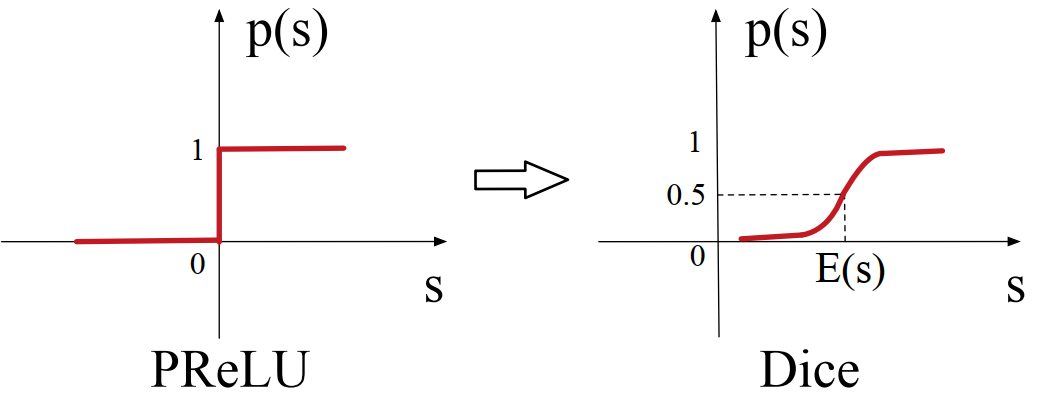
\includegraphics[width=.6\textwidth]{pics/prelu-dice.png}
	\caption{Rectified Point of PReLU and Dice}
	\label{fig:prelu_dice}
\end{figure}
Data Dependent Activation Function, Dice激活函数诞生于 DIN 中, 根据 PReLU 改造而来. ReLU 类函数的阶跃变化点在 x=0 处, 意味着面对不同的输入这个变化点是不变的, PReLU 和 Dice 的阶跃点比较如 Fig.\ref{fig:prelu_dice} 所示. DIN 中改进了这个变化点的位置, 让它根据数据的分布(神经元输出的均值和方差, 与 BN 类似)自适应来调整阶跃点的位置: 
$$
dice(x) = p(x) \cdot x + (1 - p(x)) \cdot \alpha \cdot x
$$
其中 $p(x) = sigmoid( BN(x))$, $BN(x) = \frac{x - E(x)}{\sqrt{Var(x) + \epsilon}}$. 与 PReLU 相比, 其实相当于将 max/min 这种硬的划分改成了软(即以概率 $p(x)$)的划分. 从公式和 Fig.\ref{fig:prelu_dice} 中可以看出, 均值控制了阶跃点的位置, 方差控制了阶跃处的变化速率, 即斜率. 

\subsubsection{Softplus}
Softplus 函数可以看作是 ReLU 函数的平滑, 即 $x^+ = max(0, x)$ 的平滑, 因此叫做 Softplus. 形式为: 
$$
Softplus(x) = log(1+e^x)
$$
显然, Softplus 输出的值域是 $(0, +\infty)$. 

\subsection{学习率调整策略}
\paragraph{WHY?}学习率 (Learning Rate, LR) 是基于梯度下降的优化算法中不可或缺的一部分, 目前的深度学习模型无一不使用梯度来优化模型参数, 设置学习率是不可避免的. 在训练过程中, 学习率是否应该变化, 应该如何变化对模型的收敛效果有很大的影响. 看看LR对学习过程的影响: 
\begin{myitemize}
	\item 学习率设置太小, 需要花费过多的时间来收敛
	\item 学习率设置较大, 在最小值附近震荡却无法收敛到最小值
	\item 进入局部极值点
	\item 停在鞍点处, 不能够在另一维度继续下降
\end{myitemize}

\paragraph{哪些策略}总体来说, LR可以是固定的, 即整个训练过程中不变; 也可以是动态的, 即在训练时变化, 当让根据不同的变化方式动态策略又有多种. 
\begin{myitemize}
	\item 固定LR, 整个训练过程中LR保持不变. 固定LR适用于优化目标为凸函数的情况, 当为非凸时可能会收敛到局部极值点然后开始振荡. 且LR的大小选择很重要, 为了保证收敛一般会设置的比较小. 
	\item LR衰减 (LR Decay) , 即LR随着训练进程而减小. 在训练初期大步长向目标前进, 后期小碎步靠近最优点. 常见的衰减策略: 
	\begin{myitemize}
		\item 固定步长衰减, 即每隔一定步数/epoch数, 就对LR衰减一次
		\item 指数形式衰减, 即以指数形式衰减, 通常是$LR = LR \times \gamma^{n}$, 其中$\gamma$由用户指定, $n$可以是\textit{step}或\textit{epoch}
		\item 多步长衰减, 即在不同的区间使用不同的LR. 通常是设置一系列的epoch锚点, 达到锚点后LR就衰减一次, 因此也要设置$\gamma$
	\end{myitemize}
	\item 基于Armijo准则步长搜索算法, 遵循两个准则搜索步长: 1) 目标函数值下降幅度要大于一定阈值; 2) 搜索的步长不应该太小. 这种步长调整策略较为耗时
	\item 循环学习率, 即LR的变化呈现周期性, 当然也可以每过一个周期LR就衰减一次
	\item 自适应学习率, 即自定义一些规则来决定学习率的如何改变
	\item 不同的网络层使用不同的LR
\end{myitemize}
以上这些LR调整策略只是简单介绍了调整策略的思想, 在实践中, 深度学习框架一般会提供一些LR调整策略的接口, 也可以自定义调整策略. 

参考资料: \href{https://lumingdong.cn/setting-strategy-of-gradient-descent-learning-rate.html}{梯度下降学习率的设定策略}. 
